\documentclass[10pt]{article}
\usepackage[margin=1.8cm]{geometry}
\usepackage{amsmath,amssymb,booktabs,graphicx}
\usepackage[hidelinks]{hyperref}
\setlength{\parindent}{0pt}
\setlength{\parskip}{3pt}
\newcommand{\E}{\mathbb{E}}
\title{Two-score settings with a continuous outcome}
\author{Claude, for the author \quad (exploratory; 2026-10-28)}
\date{}

\begin{document}
\maketitle
\vspace{-2em}

\section*{Common model and estimator}

Each setting has two scores $Q=(Q_1,Q_2)$, covariates $X$, a continuous outcome $Y$, and a
deployed rule $D=\mathbf 1\{Q\in A_0\}$ that the data reproduce exactly. The model is
\begin{align*}
 Q_j &= \gamma_j^\top \tilde X+\eta_j,\quad j=1,2,\qquad X\perp\eta=(\eta_1,\eta_2),\qquad T_j=\gamma_j^\top\tilde X,\\
 Y &= b(\eta)+X^\top\beta_1+D\{\alpha(\eta)+X^\top\beta_2\}+\varepsilon,\qquad \E(\varepsilon\mid D,X,\eta)=0 .
\end{align*}
For a rule $A$ the target is the supported utility
\[
 U(A)=\E\bigl[I(\eta)\{\alpha(\eta)-c+X^\top\beta_2\}\mathbf 1\{T+\eta\in A\}\bigr],\qquad
 I(\eta)=\mathbf 1\{\epsilon\le \pi_0(\eta)\le 1-\epsilon\},\quad \pi_0(\eta)=P(T+\eta\in A_0),
\]
the gain in $Y$ per unit from treating the units the rule selects, counted only where the
deployed rule gives overlap. Here $c=0$ and $\epsilon=0.05$. Rule classes: the weighted
sum $\lambda Q_1+(1-\lambda)Q_2\ge\phi$ with the deployed weight (only $\phi$ moves) or a
chosen weight; a cutoff on each score with both required ($Q_1\ge\phi_1$ and
$Q_2\ge\phi_2$); and with either enough.

\textbf{Estimator} (\texttt{experiments/methods/two\_score.py}). Four folds with four roles
(first stage, outcome, index, evaluation), rotated. OLS of each score on $X$; $\hat\alpha$
and $\hat b$ are tensor-product cubic splines in $(\eta_1,\eta_2)$ with a second-difference
penalty chosen by 5-fold cross-validation, and $X$ enters linearly in each arm;
$\hat U(A)$ is the pairwise average over $\hat\eta_i$ (evaluation fold) and
$(\hat T_j,X_j)$ (index fold). Each rotation maximizes $\hat U$ over each class; the
reported rule is the average of the four. \emph{No bootstrap here}: the range over the
four rotations is shown as a rough gauge of stability, not a confidence interval.
In simulations the feasible estimator is root-$n$ from about $n=64$k, with a variance
20--40 times the oracle's.

\textbf{Figures} (one panel set per setting; averages over the four rotations):
(a) $\hat\alpha(\eta)$, the effect at the covariate mean, drawn only where $\hat U$ counts
(inside the trim, dashed) and where there are data, with the density of $\hat\eta$ in grey
and $\hat\alpha=0$ solid; (b) $\hat U(\phi)$ with the deployed weights; (c)
$\hat U(\lambda,\phi)$; (d) $\hat U(\phi_1,\phi_2)$ for both cutoffs. $\hat U$ is in units
of $Y$ per unit of the evaluation fold.

\textbf{Settings} (one per page): Texas A/B; Florida B/C; North Carolina B/C; North
Carolina low-performing designation; NYC Progress Reports A/B.

\textbf{Left out.} Binary outcomes (Chile enrollment, gainful-employment closure, bank
failure). Settings where every rule class went to the edge of its range because the
estimated effect is flat, null or too noisy: Wisconsin, California Dashboard, CMS hospital
penalty, dialysis payment cuts, nursing-home staffing, FDIC capital (loan growth; banks
also bunch at the cutoffs), census tracts, NYC C/D. Too small for four folds: Louisiana
($n=1{,}089$), Indiana ($2{,}590$).

\textbf{Common caveats.} $X\perp\eta$ fails in every setting (the noise is heteroskedastic
in $T$); schools repeat across years; and for schools, next year's score reuses some of
this year's test data. The effect is identified only on the trimmed region, near the
deployed boundary.

Code: \texttt{experiments/scripts/two\_score\_writeup.py} (figures, \texttt{numbers.json});
datasets under \texttt{experiments/datasets/}.

%-------------------------------------------------------------------------------------
\newpage
\section*{1. Texas A--F campus ratings: the A/B boundary}

\textbf{Data.} TEA campus ratings, 2019 and 2022--2025; non-alternative campuses with all
three domain scores, outside the four districts with local accountability; $n=38{,}075$
campus-years, 22.5\% rated A (\texttt{tx\_school\_ratings}).

\textbf{Scores.} $Q_1=M=\max(\text{Student Achievement},\text{School Progress})$ and
$Q_2=$ Closing the Gaps, each a scaled score 0--100.
\textbf{Deployed rule.} A if $\operatorname{round}(0.7M+0.3\,\mathrm{CtG})\ge 90$, i.e.\
$0.7Q_1+0.3Q_2\ge 89.5$ (reproduces every published score outside the local-accountability
districts).
\textbf{$X$} (34 columns): \% economically disadvantaged, \% emergent bilingual, log
students, lowest and highest grade, charter, school type, district log enrollment and \%
disadvantaged, ESC region, year.
\textbf{$Y$}: the next rated year's overall scaled score (sd 10.4).

\textbf{Fit.} $R^2$ of $Q$ on $X$: 0.37, 0.30; $\operatorname{corr}(\hat\eta_1,\hat\eta_2)=0.73$;
66\% of evaluation units inside the trim. In the trimmed region $\hat\alpha$ ranges from
$-29$ to $3.9$ (mean $-1.3$; positive for 37\%); $\operatorname{sd}(X^\top\hat\beta_2)=2.3$.

\begin{center}\small
\begin{tabular}{lllll}
\toprule
class & deployed & estimate & 4 rotations & $\hat U$ (deployed 0.272)\\
\midrule
weights fixed (0.7, 0.3) & $\phi=89.5$ & $\phi=87.9$ & 87.0--88.9 & 0.281\\
weights chosen & $(0.7, 89.5)$ & $(0.56, 87.3)$ & $\lambda$ 0.40--0.75; $\phi$ 86.8--88.5 & 0.287\\
both cutoffs & -- & $(86.8, 82.0)$ & $\phi_1$ 85.7--88.0; $\phi_2$ 79.1--83.7 & 0.294\\
either cutoff & -- & unstable & 3 of 4 rotations at the edge & 0.270\\
\bottomrule
\end{tabular}
\end{center}

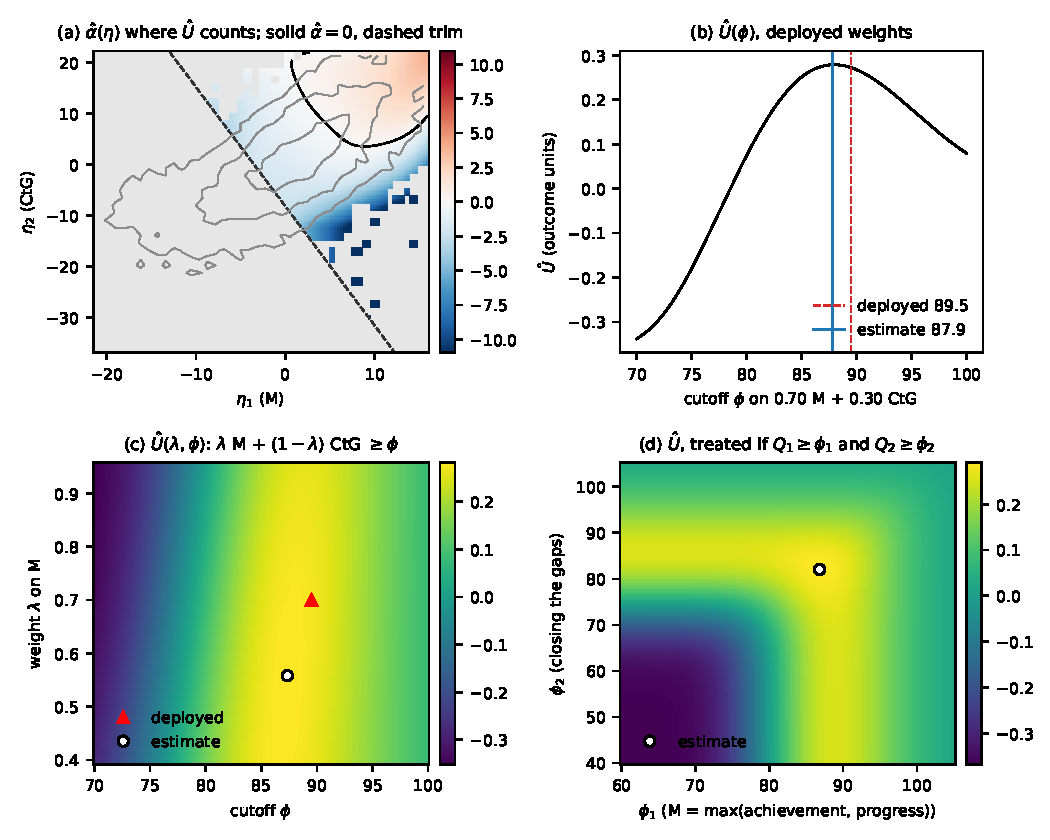
\includegraphics[width=\textwidth]{figures/tx_school_ratings.pdf}

\textbf{Reasonable?} The rule is reproduced exactly and the sample is the largest of the
school settings. $\hat U(\phi)$ has a clear interior peak 1.6 points below the deployed
cutoff, and the both-cutoffs optimum is stable across rotations. But the gain is
about 0.01--0.02 points of a score with sd 10.4, the weight is poorly determined ($\hat U$
is flat in $\lambda$, panel c), and the large negative $\hat\alpha$ sits in a sparse
corner. The 2023 and 2024 ratings were published after the next year's tests.

%-------------------------------------------------------------------------------------
\newpage
\section*{2. Florida school grades: the B/C boundary (elementary)}

\textbf{Data.} FLDOE school grades, 2017--2019 and 2022; elementary schools graded on
exactly seven components; $n=6{,}940$ school-years, 56\% graded B or better
(\texttt{fl\_school\_grades}, \texttt{load\_two\_score}).

\textbf{Scores.} $Q_1=$ mean of ELA, math and science achievement (\%), $Q_2=$ mean of the
four learning-gains components (\%).
\textbf{Deployed rule.} B or better if the percent of points
$(3Q_1+4Q_2)/7\ge 53.5$ (published grades match for every school).
\textbf{$X$} (73 columns): \% economically disadvantaged, \% minority, log enrollment,
charter, Title I, collocated, district, year.
\textbf{$Y$}: next year's percent of points (sd 13.3).

\textbf{Fit.} $R^2$: 0.72, 0.35; $\operatorname{corr}(\hat\eta)=0.53$; 89\% inside the
trim. Cross-validation picks the top of the penalty grid in every rotation, so
$\hat\alpha$ is close to bilinear: from $-8.8$ to $5.2$ (mean 0.3; positive for 59\%);
$\operatorname{sd}(X^\top\hat\beta_2)=5.7$.

\begin{center}\small
\begin{tabular}{lllll}
\toprule
class & deployed & estimate & 4 rotations & $\hat U$ (deployed 1.592)\\
\midrule
weights fixed (3/7, 4/7) & $\phi=53.5$ & $\phi=53.6$ & 49.8--56.1 & 1.629\\
weights chosen & $(0.43, 53.5)$ & $(0.31, 53.6)$ & $\lambda$ 0.22--0.43; $\phi$ 50.3--56.0 & 1.649\\
both cutoffs & -- & $(38.8, 50.9)$ & $\phi_1$ 20--55 (unstable); $\phi_2$ 48.1--53.8 & 1.570\\
either cutoff & -- & $(61.4, 56.3)$ & $\phi_1$ 56.7--65.7; $\phi_2$ 52.6--60.5 & 1.620\\
\bottomrule
\end{tabular}
\end{center}

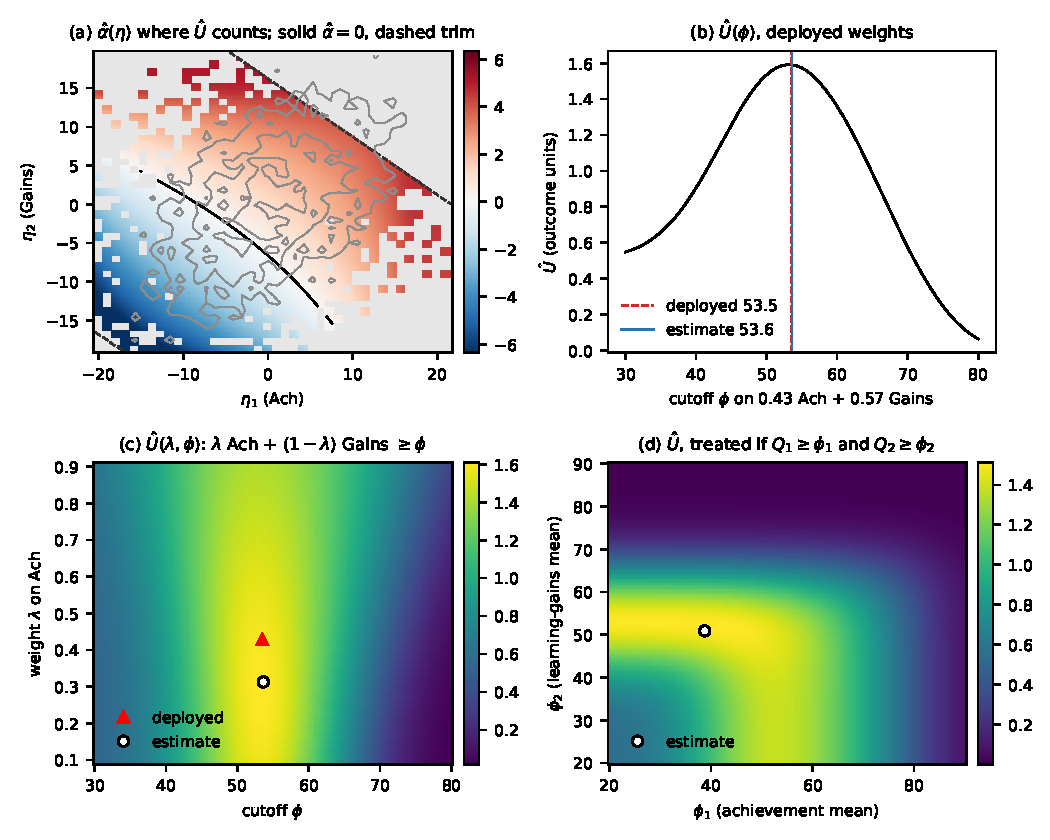
\includegraphics[width=\textwidth]{figures/fl_school_grades.pdf}

\textbf{Reasonable?} The estimated cutoff equals the deployed one, and the chosen weight
puts more weight on learning gains (0.69 against 0.57). The rotations spread over
6 points, and the sample is small for four folds. With the penalty at the top of the
grid the effect surface is essentially a plane, so the shape in panel (a) is imposed
more than estimated. I have not checked whether the trim, which is centred on the
deployed boundary, pulls the estimate toward it.

%-------------------------------------------------------------------------------------
\newpage
\section*{3. North Carolina school performance grades: the B/C boundary}

\textbf{Data.} NC DPI school performance grades, 2018--2025; $n=12{,}425$ school-years,
29.9\% graded B or better (\texttt{nc\_school\_grades}).

\textbf{Scores.} $Q_1=$ achievement score, $Q_2=$ growth score (0--100).
\textbf{Deployed rule.} B or better if $0.8Q_1+0.2Q_2\ge 69.5$ (100\% of published grades).
\textbf{$X$} (129 columns): \% economically disadvantaged, race shares, English learners,
students with disabilities, log ADM and its change, \% inexperienced teachers, charter,
Title I, calendar, school type and special types, district, year.
\textbf{$Y$}: next year's school performance score (sd 14.4).

\textbf{Fit.} $R^2$: 0.79 for achievement but 0.11 for growth;
$\operatorname{corr}(\hat\eta)=0.41$; 96\% inside the trim. $\hat\alpha$ from $-4.9$ to
$1.6$ (mean $-1.0$; positive for 26\%); $\operatorname{sd}(X^\top\hat\beta_2)=4.4$.

\begin{center}\small
\begin{tabular}{lllll}
\toprule
class & deployed & estimate & 4 rotations & $\hat U$ (deployed 0.490)\\
\midrule
weights fixed (0.8, 0.2) & $\phi=69.5$ & $\phi=69.5$ & 66.8--72.5 & 0.498\\
weights chosen & $(0.8, 69.5)$ & $(0.88, 68.4)$ & $\lambda$ 0.75--0.95 (2 at edge); $\phi$ 64.3--73.1 & 0.505\\
both cutoffs & -- & $(66.7, 50.3)$ & $\phi_1$ 63.5--69.4; $\phi_2$ 39.9--68.1 & 0.502\\
either cutoff & -- & achievement only & growth cutoff at the edge in all 4 & 0.486\\
\bottomrule
\end{tabular}
\end{center}

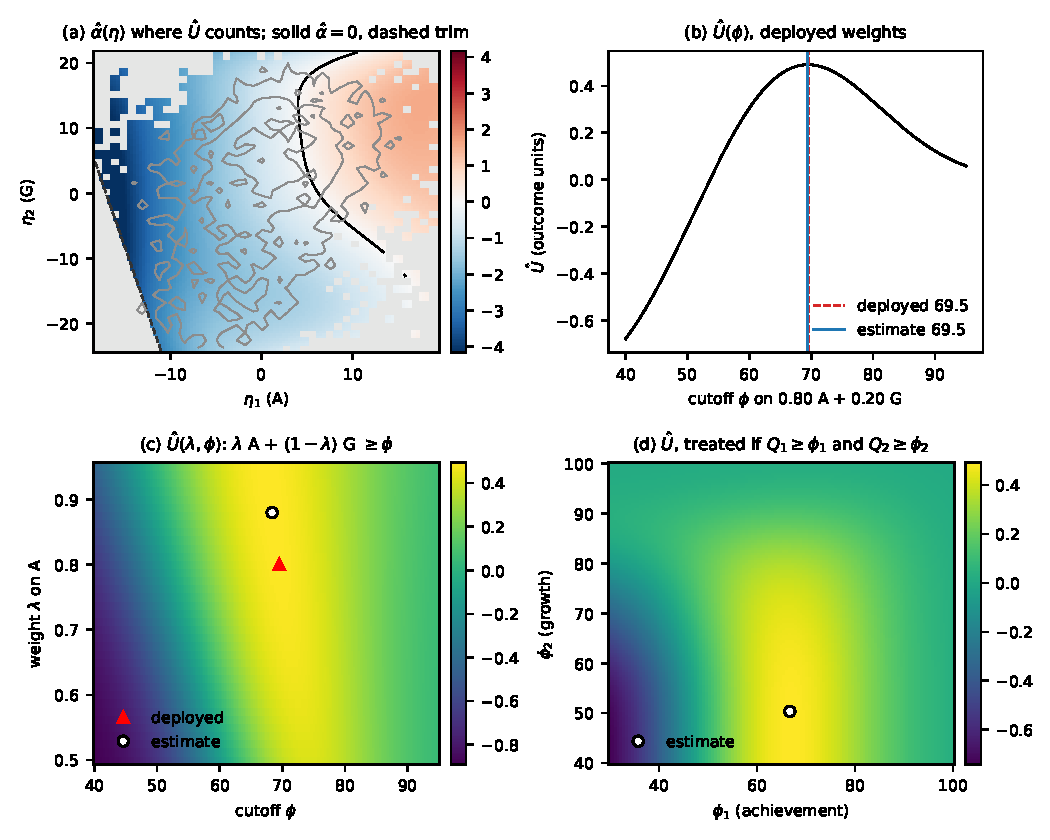
\includegraphics[width=\textwidth]{figures/nc_school_grades.pdf}

\textbf{Reasonable?} The rule and sample are clean, but the estimate is the deployed
cutoff with a 6-point rotation range, the gain is 0.01 points, and every class that can
move the growth cutoff pushes it out of play. Growth is nearly unpredictable from $X$
($R^2=0.11$), so $T$ has little spread in that direction and the trade-off between the
scores is weakly identified.

%-------------------------------------------------------------------------------------
\newpage
\section*{4. North Carolina low-performing designation (both cutoffs)}

\textbf{Data.} As in setting 3; $n=12{,}425$ school-years, 26.5\% designated
(\texttt{nc\_school\_grades}, \texttt{load\_low\_performing}).

\textbf{Scores.} $Q_1=0.8A+0.2G$ (the school performance score), $Q_2=$ growth $G$.
\textbf{Deployed rule.} Designated low-performing if $Q_1<54.5$ \emph{and} $Q_2<85$ (a
both-cutoffs rule on the low side; reproduces all 4,055 designations). Designation brings
a required improvement plan and district and state support.
\textbf{$X$}, \textbf{$Y$}: as in setting 3. $D=1$ is designation.

\textbf{Fit.} $R^2$: 0.74, 0.11; $\operatorname{corr}(\hat\eta)=0.64$; 84\% inside the
trim. $\hat\alpha$ from $-2.2$ to $2.8$ (mean $-0.3$; positive for 34\%), positive for
schools whose score is below what $X$ predicts ($\eta_1<-5$) and negative above;
$\operatorname{sd}(X^\top\hat\beta_2)=4.6$.

\begin{center}\small
\begin{tabular}{lllll}
\toprule
class & deployed & estimate & 4 rotations & $\hat U$ (deployed 0.413)\\
\midrule
both cutoffs & $(54.5, 85)$ & $Q_1<59.6$ and $Q_2<90.0$ & $\phi_1$ 52.9--73.3; $\phi_2$ 86.2--99.2 & 0.494\\
either cutoff & -- & unstable & 3 of 4 rotations at the edge & 0.489\\
\bottomrule
\end{tabular}
\end{center}

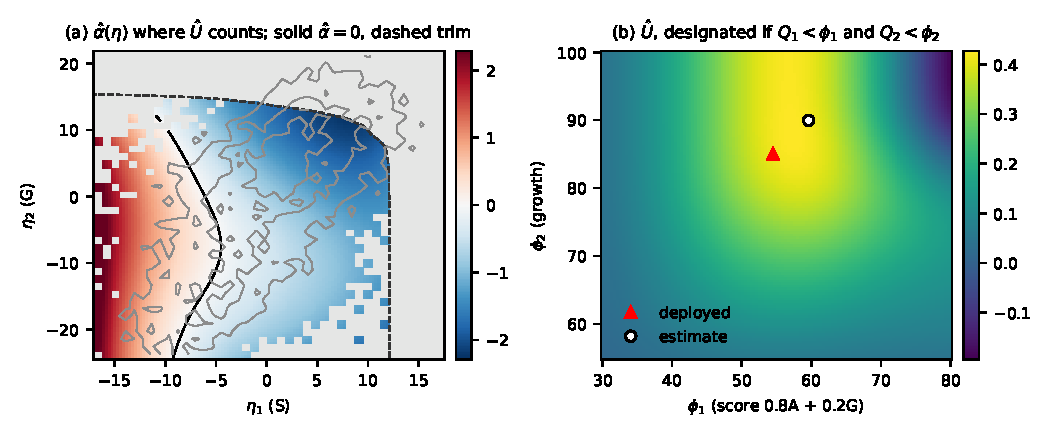
\includegraphics[width=\textwidth]{figures/nc_low_performing.pdf}

\textbf{Reasonable?} This is the setting where $\hat\alpha$ changes sign inside the data
in an interpretable way: designation helps the schools that score far below their
predicted level and hurts the others. $\hat U$ has a clear ridge (panel b) and the
estimate would designate more schools than the deployed rule. Three of the four
rotations agree on $(53$--$58, 86$--$88)$; the fourth drifts to $(73, 99)$. The gain,
0.08 points, is the largest relative to $Y$ among the five settings, but still small.

%-------------------------------------------------------------------------------------
\newpage
\section*{5. NYC Progress Reports: the A/B boundary}

\textbf{Data.} NYC DOE Progress Reports for elementary, K-8 and middle schools, rating
years spring 2008--2012; $n=5{,}348$ school-years, 39.4\% graded A
(\texttt{nyc\_progress\_reports}, \texttt{load\_two\_score("AB")}).

\textbf{Scores.} With $c$ the year's published cut for the school type,
$Q_1=100(\text{Environment}+\text{Performance}+\text{credit}-0.4c)/40$ and
$Q_2=100(\text{Progress}-0.6c)/60$: each in percent of its category maximum, net of its
share of the cut.
\textbf{Deployed rule.} A if $0.4Q_1+0.6Q_2\ge 0$ (every published A/B grade).
\textbf{$X$} (62 columns): poverty, ELL, special-education, race and male shares, log
enrollment, tested share, the DOE peer indices, last year's percentile, school type,
charter, community district, year (missing-value flags).
\textbf{$Y$}: next year's overall score (sd 19.4).

\textbf{Fit.} $R^2$: 0.52, 0.31; $\operatorname{corr}(\hat\eta)=0.55$; 85\% inside the
trim. $\hat\alpha$ from $-13.8$ to $4.2$ (mean $-2.0$; positive for 20\%);
$\operatorname{sd}(X^\top\hat\beta_2)=7.5$.

\begin{center}\small
\begin{tabular}{lllll}
\toprule
class & deployed & estimate & 4 rotations & $\hat U$ (deployed 0.746)\\
\midrule
weights fixed (0.4, 0.6) & $\phi=0$ & $\phi=4.6$ & $-0.9$--12.4 & 0.839\\
weights chosen & $(0.4, 0)$ & $(0.20, 2.4)$ & $\lambda$ 0.10--0.30; $\phi$ $-4.1$--9.9 & 0.882\\
both cutoffs & -- & $(-21.4, 0.1)$ & $\phi_1$ $-38$ to $-4$; $\phi_2$ $-6.7$--10.1 & 0.871\\
either cutoff & -- & unstable & $\phi_1$ 29--60 & 0.859\\
\bottomrule
\end{tabular}
\end{center}

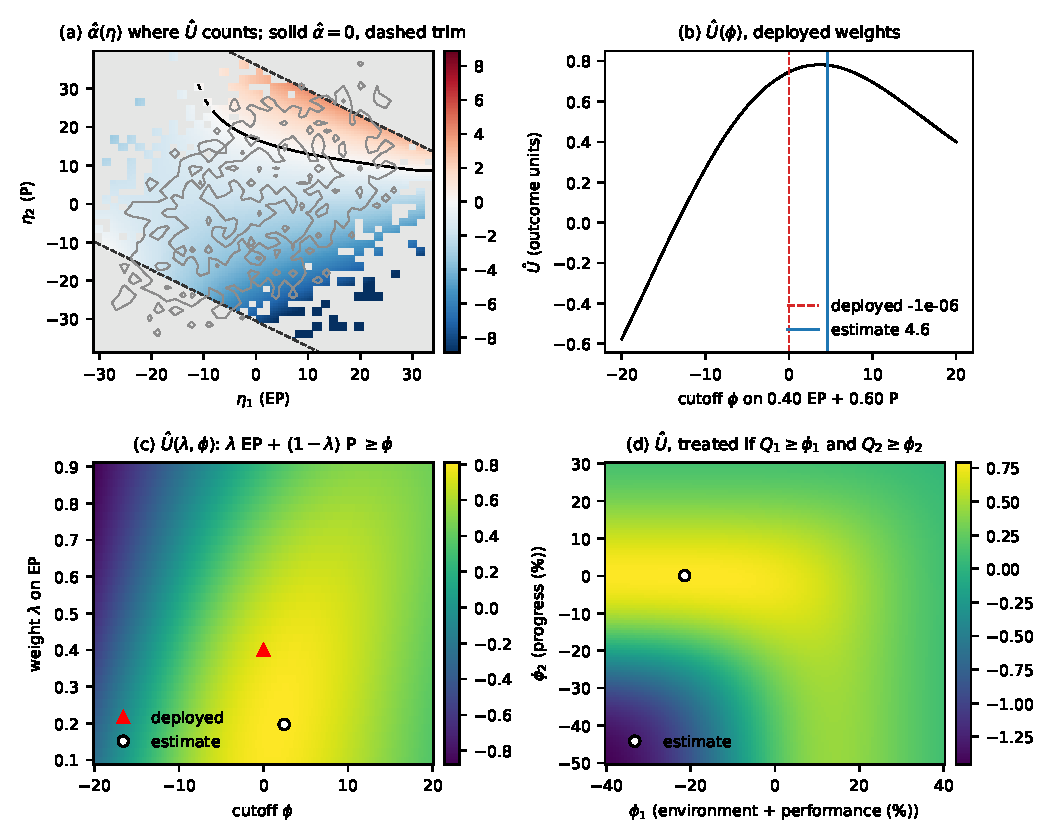
\includegraphics[width=\textwidth]{figures/nyc_progress_reports_ab.pdf}

\textbf{Reasonable?} The direction is consistent across rotations: a higher A cutoff and
more weight on progress (the chosen $\lambda$ is 0.1--0.3 in every rotation). But the
cutoff ranges over 13 points, $n$ is small, and from 2009--10 the A share was fixed by design each year
(the cut was set at a percentile), so a ``different cutoff'' also means a different A
share. The category scores are percentile-based, and the metrics changed in 2009--10.

\end{document}
